\section{User interface}

The following will explain the structure of the user interface. 

%\subsection{Splash screen}

%\begin{minipage}{0.45\textwidth}
%When the app is launched and until it is fully loaded, a splash screen shows the app's logo.
%\end{minipage} \hfill
%\begin{minipage}{0.5\textwidth}
%\framebox{
\includegraphics[scale=0.4]{pics/GUI/01-GUI-startup.png}}
%\end{minipage}

\subsection{Start screen}

\begin{minipage}{0.45\textwidth}
When the app is fully loaded, the main menu is shown. It provides an overview of the three main functionalities of the app. This way, the user can choose directly what they want to do first:
Either to record new data (and afterwards view them via the web application which can be invocated from here), to view the live data or to enter the settings screen where the tracking can be configured and the sensor device can be scanned for and connected to.
\end{minipage} \hfill
\begin{minipage}{0.5\textwidth}
\framebox{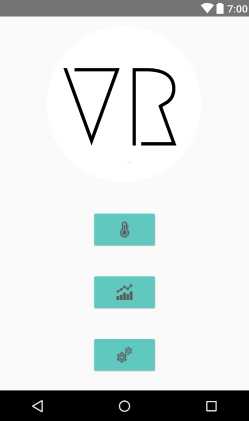
\includegraphics[scale=0.4]{pics/GUI/main.png}}
\end{minipage}

\subsection{Record Data}

\begin{minipage}{0.3\textwidth}
Here, the user can start a new recording session and view the data that have been collected so far.
\end{minipage} \hfill
\begin{minipage}{0.3\textwidth}
\framebox{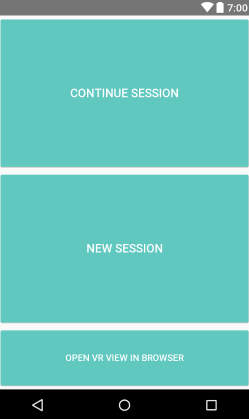
\includegraphics[scale=0.4]{pics/GUI/record.png}}
\end{minipage}
\begin{minipage}{0.3\textwidth}
\framebox{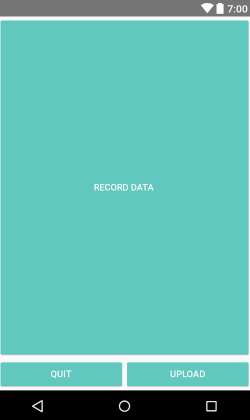
\includegraphics[scale=0.4]{pics/GUI/session.png}}
\end{minipage}


\subsection{3D View}

\begin{minipage}{0.45\textwidth}
When the 3D view is chosen, the web application is started automatically.
\end{minipage} \hfill
%\begin{minipage}{0.5\textwidth}
%\framebox{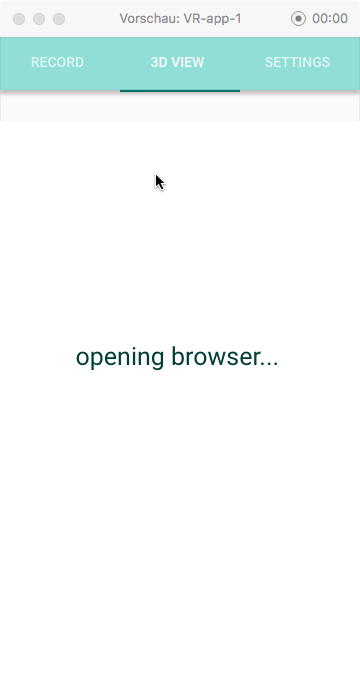
\includegraphics[scale=0.4]{pics/GUI-entwurf/04-GUI-VR.png}}
%\end{minipage}

\subsection{Settings}

\begin{minipage}{0.45\textwidth}
Here, the tracking can be configured and the sensor device can be searched for and also be configured.
\end{minipage} \hfill
\begin{minipage}{0.5\textwidth}
\framebox{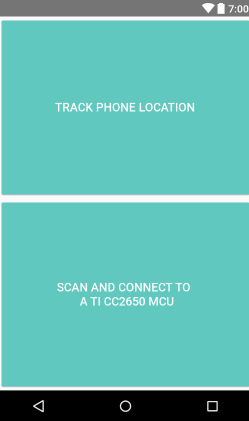
\includegraphics[scale=0.4]{pics/GUI/settings.png}}
\end{minipage}
